\documentclass[onehalfspace]{USB}
\usepackage{paralist}
\usepackage{natbib}
% \usepackage[figuresright]{rotating}
\usepackage{lscape}
\usepackage{graphicx}
\usepackage{longtable}
\usepackage{calc}
% \usepackage{slashbox}
\usepackage{adjustbox}
\usepackage{amsmath}
\usepackage{amsfonts}
\usepackage{amssymb}
% \usepackage{setspace}
\usepackage{color}
\usepackage{geometry}
% \usepackage[none]{hyphenat}
% \usepackage{layouts}
\usepackage{blindtext}
\graphicspath{ {Imagenes/} }
%------------------------------------------------------------------------------%


%------------------------------------------------------------------------------%
%                                                                              %
%                                    MÁRGENES                                  %
%                                                                              %
%------------------------------------------------------------------------------%

\geometry{
  reset,
  letterpaper,
  left=3cm,
  right=2cm,
  top=2cm, 
  bottom=2cm
}

\begin{document}
\frontmatter
%------------------------------------------------------------------------------%

% \drawdimensionstrue
% \printinunitsof{cm}
% \pagevalues
% \currentpage
%%%%%%%%%%%%%%%%%%%%%%%%%%%%%%%%%%%%%%%%%%%%%%%%%%%%%%%%%%%%%%%%%%%%%%%%%
%                                                                       %
%                               CARÁTULA                                %
%                                                                       %
%%%%%%%%%%%%%%%%%%%%%%%%%%%%%%%%%%%%%%%%%%%%%%%%%%%%%%%%%%%%%%%%%%%%%%%%%
\thispagestyle{empty}
\begin{center}
    \begin{singlespace}
        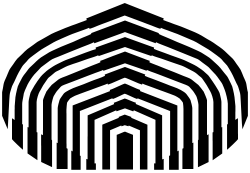
\includegraphics[width=2cm]{logo_USB}
        
        {\large
          UNIVERSIDAD SIMÓN BOLÍVAR\\
        }
        
        \textbf{
          DECANATO DE ESTUDIOS PROFESIONALES\\
          COORDINACIÓN DE INGENIERÍA DE LA COMPUTACIÓN
        }
        
        \vspace{4cm}%
        \textbf{
          DESARROLLO DEL MÓDULO PRINCIPAL Y ESTADÍSTICAS DE LA LIBRERÍA AUDITORÍAS TURPIAL
        }
        \vspace{4cm}
        
        Por:\\
        Stefani Carolina Castellanos Torres
        
        \vspace{5cm}
          \textbf{INFORME DE PASANTÍA}\\
          Presentado ante la Ilustre Universidad Simón Bolívar\\
          como requisito parcial para optar al título de\\
          Ingeniero de la Computación\\
        \selectfont
        
        \vspace{3cm}
        Sartenejas, Enero 2018
    
    \end{singlespace}
\end{center}

\clearpage

%%%%%%%%%%%%%%%%%%%%%%%%%%%%%%%%%%%%%%%%%%%%%%%%%%%%%%%%%%%%%%%%%%%%%%%%%
%                                                                       %
%                               PORTADA                                 %
%                                                                       %
%%%%%%%%%%%%%%%%%%%%%%%%%%%%%%%%%%%%%%%%%%%%%%%%%%%%%%%%%%%%%%%%%%%%%%%%%

\thispagestyle{empty}

\begin{center}
    \begin{singlespace}
        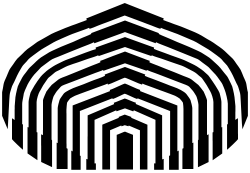
\includegraphics[width=2cm]{logo_USB}
        
        {\large
          UNIVERSIDAD SIMÓN BOLÍVAR\\
        }
        
        \textbf{
          DECANATO DE ESTUDIOS PROFESIONALES\\
          COORDINACIÓN DE INGENIERÍA DE LA COMPUTACIÓN
        }
        
        \vspace{4cm}%
        \textbf{
          DESARROLLO DEL MÓDULO PRINCIPAL Y ESTADÍSTICAS DE LA LIBRERÍA AUDITORÍAS TURPIAL
        }
        \vspace{4cm}
        
        Por:\\
        Stefani Carolina Castellanos Torres
        
        \vspace{1cm}
        Realizado con la asesoría de:\\
        Tutor Académico: MSc. Angela Di Serio\\
        Tutor Industrial: Ing. Pedro Romero
        
        \vspace{2cm}
          \textbf{INFORME DE PASANTÍA}\\
          Presentado ante la Ilustre Universidad Simón Bolívar\\
          como requisito parcial para optar al título de\\
          Ingeniero de la Computación\\
        \selectfont
        
        \vspace{3cm}
    Sartenejas, Enero 2018
    
    \end{singlespace}
\end{center}




%------------------------------------------------------------------------------%
\addcontentsline{toc}{chapter}{\textbf{RESUMEN}}
\begin{center}
    \vspace{2cm}
    \textbf{
    DESARROLLO DEL MÓDULO PRINCIPAL Y ESTADÍSTICAS DE LA LIBRERÍA AUDITORÍAS TURPIAL
    }

    \vspace{2cm}

    Por:\\
    Stefani Carolina Castellanos Torres

    \vspace{2cm}

    \textbf{RESUMEN}\\

    \vspace{2cm}

\end{center}

Auditorías Turpial es una librería para Django que permite mantener un historial de las operaciones realizadas sobre alguna tabla de base de datos, a través de auditorías. La empresa Turpial Development, requiere una librería de Django que le permita acelerar el desarrollo de aplicaciones que necesiten un sistema de este tipo, y esté desarrollado bajo la arquitectura de microservicios para que sea fácil de integrar. Esta librería consta de tres módulos: Principal (\textit{Core}), Estadísticas y Reportes. Adicionalmente, estos microservicios pueden ser actualizados mediante una herramienta de Integración Continua. En el presente informe se describen los procesos de diseño, implementación y pruebas de parte del módulo \textit{Core} y completamente el módulo Estadísticas de Auditorías Turpial, desarrollado como pasantía larga en Turpial Development siguiendo la metodología \textit{Turpial Agile Unified Process}. Así como, la implantación del sistema de Integración Continua utilizando Jenkins. Como resultado, se lograron todos los objetivos planteados y otros originados durante la fase de construcción. \\

    \textbf{Palabras claves}: Auditoría de sistemas, librería, Django, Integración Continua, microservicio.


%------------------------------------------------------------------------------%
% \addcontentsline{toc}{chapter}{\textbf{DEDICATORIA}}
\chapter*{DEDICATORIA}

\begin{flushright}
    \textit{
        "Es mucho más difícil juzgarse a sí mismo, que juzgar a los otros. Si consigues juzgarte rectamente es que eres un verdadero sabio."
    }
    - Antoine de Saint-Exupéry. El Principito
    \vspace{2cm}
    \textit{"No vivas imaginando problemas que no han ocurrido ni van a suceder; disfruta del presente, la vida hay que aprovecharla, elige siempre poner en tu mente lo agradable en lugar de lo desagradable."
    }
    ― Enrique Barrios. Ami, el niño de las estrellas.

\end{flushright}


%------------------------------------------------------------------------------%
% \addcontentsline{toc}{chapter}{\textbf{RECONOCIMIENTOS Y AGRADECIMIENTOS}}
\chapter*{RECONOCIMIENTOS Y AGRADECIMIENTOS}


%------------------------------------------------------------------------------%

%%%%%%%%%%%%%%%%%%%%%%%%%%%%%%%%%%%%%%%%%%%%%%%%%%%%%%%%%%%%%%%%%%%%%%%%%
%                                                                       %
%                               ÍNDICES                                 %
%                                                                       %
%%%%%%%%%%%%%%%%%%%%%%%%%%%%%%%%%%%%%%%%%%%%%%%%%%%%%%%%%%%%%%%%%%%%%%%%%


\addcontentsline{toc}{chapter}{\textbf{ÍNDICE}}
\tableofcontents
\listoftables
\listoffigures
\newpage
\addcontentsline{toc}{chapter}{\textbf{LISTA DE SÍMBOLOS}}
\chapter*{LISTA DE SÍMBOLOS}

símbolos
\newpage
\addcontentsline{toc}{chapter}{\textbf{LISTA DE ABREVIACIONES}}
\chapter*{LISTA DE ABREVIACIONES}
%%%%%%%%%%%%%%%%%%%%%%%%%%%%%%%%%%%%%%%%%%%%%%%%%%%%%%%%%%%%%%%%%%%%%
% If abbreviations and acronyms (e.g. MARDI, UPM) are used in the   %
% thesis, they should be explained in a List of Abbreviations, even %
% though the full names are given when the terms are first          %
% mentioned in the text. This list should be the last item in the   %
% preliminary section. It serves as a ready reference to readers    %
% not familiar with the abbreviations used in the thesis.           %
% Universally recognised scientific symbols (such as cm, mm, kg)    %
% need not be listed.                                               %
%%%%%%%%%%%%%%%%%%%%%%%%%%%%%%%%%%%%%%%%%%%%%%%%%%%%%%%%%%%%%%%%%%%%%

\begin{center}
\begin{tabular}{ll}
VIM         &\hspace{2cm} Variational Iteration Method            \\
MVIM        &\hspace{2cm} Multistage Variational Iteration Method \\
ODEs        &\hspace{2cm} Ordinary Differential Equations         \\
PDEs        &\hspace{2cm} Partial Differential Equations          \\
$\lambda$   &\hspace{2cm} Lagrange Multiplier                     \\
ADM         &\hspace{2cm} Adomian Decomposition Method            \\
SADM        &\hspace{2cm} Standard Adomian Decomposition Method   \\
MADM        &\hspace{2cm} Modified Adomian Decomposition Method   \\
RK4         &\hspace{2cm} Fourth-order Runge-Kutta Method         \\
HAM         &\hspace{2cm} Homotopy Analysis Method                \\
\end{tabular}
\end{center}
\clearpage


%----------------------------------------------------------------------------------------%
\mainmatter
\addcontentsline{toc}{chapter}{\textbf{Introducción}}
\chapter*{\textbf{INTRODUCCIÓN}}

\blindtext

%----------------------------------------------------------------------------------------%
% The Command:                                                                           %
% \addtocontents{toc}{\addvspace{.5cm}}                                                  %
% must be added before each \include {chapter}                                           %
%----------------------------------------------------------------------------------------%
\addtocontents{toc}{\addvspace{.5cm}}
\chapter{\textbf{Entorno empresarial}}

\thispagestyle{empty}

En este capítulo se describe en ambiente de la empresa Turpial Development, en la cual se llevó a cabo la pasantía. Se presenta la misión, visión y estructura de la empresa, así como el cargo desempeñado por el pasante durante este período.


\section{Descripción}

Turpial Development es una empresa mediana, con 4 años en el mercado que está enfocada en el desarrollo de sistemas y aplicaciones Web y Móviles. Fundada e integrada por jóvenes venezolanos,  ofrece soluciones que cumplen con altos estándares de usabilidad, diseño y funcionalidad.

\section{Misión}

La empresa tiene como misión “prestar servicios y consultoría en diseño y desarrollo de soluciones web, a la medida del cliente, caracterizadas por una alta calidad, excelente soporte y experiencia de usuario”. (Manual para desarrolladores, 2016)


\section{Visión}

Su visión es “servir de plataforma para el desarrollo y éxito de nuevos emprendimientos en el área web”. (Manual para desarrolladores, 2016)

\section{Estructura}

En la figura 1.1 se muestra la estructura organizacional de Turpial Development, la cual está conformada por cuatro departamentos:

\subsection*{Dirección de Operaciones}

Se encarga del funcionamiento de todos los procesos de soporte de la empresa, como administración, recursos humanos, contabilidad y compras con el fin de garantizar el correcto desarrollo de los procesos principales de la empresa. 

\subsection*{Dirección de Proyectos} 

Se encarga de atender a las necesidades y requerimientos de los clientes, sirviendo de enlace con las direcciones de desarrollo y diseño para garantizar la calidad del producto o entrega. 

\subsection*{Dirección de Desarrollo} 

Se encarga de la conceptualización y desarrollo de las necesidades del cliente, implementando e integrando el diseño acordado y las funcionalidades requeridas por dicho cliente. Se divide en tres departamentos: Conceptualización, \textit{Backend} y \textit{Frontend}.

\subsection*{Dirección de Diseño}

Se encarga de la conceptualización y diseño de la interfaz gráfica de los proyectos en función de las necesidades del cliente y de la mano con las decisiones tomadas por la Dirección de Desarrollo. 

\begin{figure}
\centering
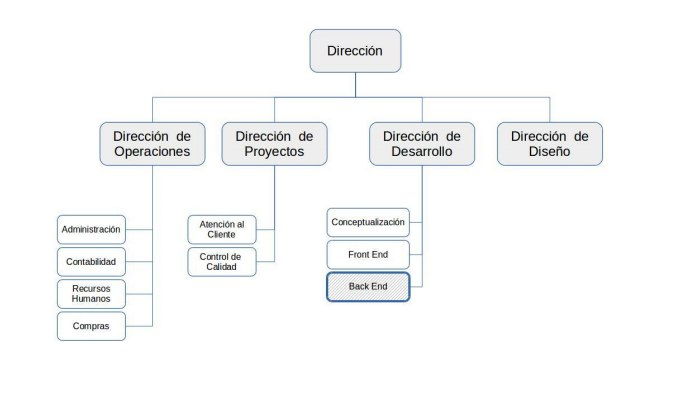
\includegraphics[width=\textwidth]{Estructura_Turpial.png}
\caption{Arquitectura de tecnologías a utilizar}
\label{fig:figure6.2}
\end{figure}

\subsection*{Ubicación del pasante}

El desarrollo de la pasantía fue llevado a cabo en la Dirección de Desarrollo de la empresa. El pasante fue asignado al departamento de \textit{Backend} bajo el cargo de Pasante, para cumplir tareas tales como: levantar requerimientos, diseñar y desarrollar las funcionalidades de la solución propuesta para el sistema. 



  % Chpater 1: Title of the chapter                                    %
\addtocontents{toc}{\addvspace{.5cm}}
\chapter{\textbf{Definición del problema}}

\thispagestyle{empty}

\section{Antecedentes}

En ocasiones, las aplicaciones necesitan un sistema que registre la creación, eliminación y actualización de los datos manejados, bien sea para cumplir estatutos gubernamentales o para observar el comportamiento de la información considerada sensible. La empresa Turpial Development desea contar con una librería confiable y de fácil instalación que provea estas funcionalidades, de manera que puedan ser ofrecidas como un servicio a sus clientes.\\

Existen algunas librería disponibles que son capaces de realizar estos procedimientos. Una de las más populares es django-reversions, una extensión de Django que provee control de versiones para los modelos del \textit{framework} y la posibilidad de restaurar la base de datos a una versión anterior. La empresa utilizó dicha librería en algunos proyectos, sin embargo, su integración delega demasiada responsabilidad al programador por lo que es susceptible a errores humanos.\\

Por otro lado, ninguna de la librerías disponibles cuentan con un módulo que permita visualizar los datos obtenidos a través de estadísticas, el desarrollador debe realizar esta labor por el mismo; Analizando la información recaudada y ajustando la estructura de datos para hacer uso de otras librerías que dispongan de la capacidad de realizar gráficas. 

\section{Planteamiento del problema}

Con el auge del desarrollo de \textit{software}, surgieron entes que controlan y supervisan el uso de la información y garantizan la confiabilidad de los mismos, por lo que algunas aplicaciones requieren mecanismos para registrar las operaciones ejecutadas. También se pueden utilizar estas trazas para caracterizar el comportamiento de alguna característica en particular del programa a desarrollar.\\

Aunque existen aplicaciones capaces de realizar estas funcionalidades, ninguna de ellas se adecúa a las necesidades de Turpial Development, ya que delegan demasiada responsabilidad a la capa lógica de la aplicación, son difíciles de entender o no registran toda la información que requieren los clientes. Es por esta razón que la empresa se vió en la necesidad de crear su propia librería que mantener un historial de acciones efectuadas sobre algunas tablas en la base de datos.

\section{Justificación}

La empresa Turpial Development decidió invertir en el desarrollo de una librería de auditorías que se ajuste tanto a las necesidades de sus programadores, como a la de sus cliente; y que agilice el desarrollo de cualquier proyecto que requiera registrar las operaciones y posea una base de datos relacional. La solución planteada es realizar dicha librería bajo la estructura de microservicio, para el \textit{framework} Django y utilizar alguna herramienta automatizada para integrar el trabajo de manera continua, empaquetar, probar y desplegar la librería de manera que se actualice con rapidez y esté disponible en todo momento.

\section{Objetivo general}

Implementar, probar y presentar las funcionalidades de selección, gestión y listados de auditorías y todas las funcionalidades del módulo Estadísticas de la librería de Auditorías Turpial e implantar un sistema de integración continua con el repositorio.  

\section{Objetivos específicos}

% \section{Citations}\label{citation}

% Please refer to the citation format listed in the file
% \emph{bibli.bib} for:
% \begin{itemize}
%     \item Article in a journal: e.g. \citep{Beth1989}.\\
%     ``Beth, T. and Gollmann, D. 1989. Algorithm Engineering for Public Key Algorithm.
%     \emph{IEEE Journal on Selected Areas in Communications} {\bf 7 (4)}:
%     458--465."
%     \item Manuscript in a conference proceedings: e.g. \citep{Burton1989}.\\
%   `` Burton, D. M. 1989. The Theory of Congruences. \emph{In Proceedings of The 22nd
%     Annual ACM Symposium on the Theory of Computation} (eds. Allyn and
%     Bacon), 80--85. The Association of Number Theory, Boston, USA:
%     Springer."
%     \item Chapter in a book: e.g. \citep{Gilbert2005}.\\
%     ``Gilbert, J. and Gilbert, L. 2005. The Integers and Congruence. \emph{In Elements of
%     Modern Algebra}, 6th edn., 57--117. New York: Thomson, Chapter 2."
%     \item Book: e.g. \citep{Hejhal1999}.\\
%     ``Hejhal, D. A., Friedman, J., Gutzwiller, M. C. and Odlyzko, A. M. 1999. \emph{Emerging
%     Applications of Number Theory}. 2nd edn. New York: Springer."
%     \item Ph.D. thesis: e.g. \citep{Whitwell2004}.\\
%     ``Whitwell, G. 2004. \emph{Novel Heuristic and Metaheuristic Approaches to
%     Cutting and Packing}. PhD thesis, School of Computer Science and
%     Information Technology. University of Nottingham."
%     \item MISC (e.g. dataset from the internet): \citep{NHSExplained}.\\
%     ``NHS Database. Retrieved 08/08/2008, Website,\\
%     \emph{http://www.nhs.uk/thenhsexplained/how the nhs works.asp}."
% \end{itemize}
  % Chapter 2: Title of the chapter                                    %
\addtocontents{toc}{\addvspace{.5cm}}
\chapter{\textbf{Marco teórico}}

\thispagestyle{empty}

En este capítulo se presentan los aspectos teóricos que sustentan y respaldan el desarrollo del proyecto de pasantía. A continuación se describen los conceptos que permiten explicar el problema planteado.

\section{Auditoría}

Es una revisión sistemática para determinar si la calidad de las actividades cumplen con los acuerdos planificados y si estos están implementados efectivamente y son adecuados para alcanzar sus objetivos. Ofrecen una oportunidad de mejora al sistema y pueden ser llevadas a cabo para cumplir con normas regulatorias. Las auditorías se pueden aplicar a sistemas, procesos, programas o servicios y pueden ser internas (realizadas por la misma empresa) o externas (realizadas por proveedores). \cite{weinstein1997total}

\section{Acciones auditables}

Se considera una acción auditable todo flujo del sistema que cree, edite o borre alguna información sensible para el mundo de negocio. Son registradas incluyendo información sobre quién realizó la acción, qué acción se intentó realizar y cuándo ocurrió la acción.

\section{Microservicio}

Es un tipo de arquitectura que consiste en desarrollar una aplicación como un conjunto de pequeños servicios. Dichos servicios son procesos autónomos, cohesivos e independientes que suelen interactuar con otros componentes a través de mensajes \cite{Microservices1}. Se enfocan en resolver un único problema y funcionan de manera aislada; si se presentan una falla no se propaga y puede ser atendido más rápidamente. \cite{Microservices2} \\

Estos servicios se manejan de manera descentralizada y hacen uso de un despliegue completamente automatizado. Cada uno de ellos pueden ser escritos en diferentes lenguajes y tecnologías para almacenar información y aún así, interactuar y compartir información. \cite{Microservices2}

\section{Integración Contínua}

Es una práctica de desarrollo de software en la que los miembros del equipo combinan su trabajo de forma periódica, usualmente cada día. Cada integración está verificada por una herramienta automatizada que empaquete y pruebe el código para detectar errores lo más rápido posible \cite{Integracion_Continua}, de esta manera se puede mejorar la calidad del software y reducir el tiempo en validar y publicar actualizaciones.

\section{Pruebas automatizadas}

Las pruebas tienen como objetivo ejercitar el código para detectar errores y verificar que el software satisface los requerimientos especificados para asegurar su calidad. Estas son realizadas desde el punto de vista del usuario y las funcionalidades son probadas ingresando información y examinando la salida. \cite{Pruebas_Automatizadas}\\ 

Esta labor puede ser larga y repetitiva, por lo que es conveniente contar con herramientas que provean métodos que faciliten el proceso de escribir y  ejecutar casos de prueba y así, reducir significativamente el esfuerzo y tiempo invertido por los desarrolladores. \cite{Pruebas_Automatizadas} A este conjunto de casos de pruebas se le conoce como prueba automatizada.

\section{Patrón Modelo-Vista-Controlador}

Este patrón de diseño asigna objetos en una aplicación a uno de tres roles: modelo, vista o controlador y define cómo se comunican entre ellos. La colección de objetos de cada tipo puede ser referido como una “capa”.\cite{MVC}

\begin{itemize}
    \item Modelo: controla el comportamiento y la data de la aplicación, responde las solicitudes de información (usualmente desde la vista) y las instrucciones de cambio de estado (usualmente desde el controlador).
    \item Vista: maneja la presentación de la información.
    \item Controlador: interpreta las entradas del usuario y le informa al modelo y/o vista para cambiar lo que sea apropiado.\cite{MVC1}
\end{itemize}



Figura 1. Diagrama del patrón MVC\\

Es importante notar que la vista y el controlador dependen del modelo, sin embargo el modelo es independiente. Esta separación permite probar el modelo aparte de la presentación visual. 

\section{Patrón Modelo-Vista-Plantilla}

Es una adaptación del patrón MVC, en el cual la “vista” define cuál dato es presentado y su comportamiento, no como se muestra. El dato es obtenido a través de la función de \textit{callback} para pedir una URL en particular. Por otro lado, la “vista” delega a la “plantilla”  la presentación de la información.\\

En el caso de Django, el “controlador” es el \textit{framework} en sí: “la maquinaria que envía una petición a la vista apropiada, de acuerdo a la configuración de URL de Django”. \cite{MVT}

\section{Señales}

Permiten a las aplicaciones ser notificadas cuando ocurra una acción en algún otro lugar, es decir, las señales permiten a ciertos emisores notificar a un conjunto de receptores que alguna acción está siendo ejecutada. \cite{Signals} En términos de \textit{software}, son el análogo a interrupciones de \textit{hardware}. \cite{Senales}

\section{Mixins}

Es un estilo de programación en el cual las unidades de funcionalidad son creadas en una clase y se incorporan en otras \cite{Mixins}. Pueden entenderse como “un subclase abstracta que puede ser usada para especializar el comportamiento de una variedad de padres”.  \cite{Mixins2} \\

Usualmente, los \textit{Mixins}, definen nuevos métodos que realizan alguna acción y luego llaman a los métodos del padre correspondiente; pueden utilizarse en varias clases de la jerarquía y sin importar en qué clases sean usadas. \\

Hay varias razones para usar \textit{Mixins}: extienden las clases existentes sin tener que editar, mantener o combinar el código fuente; mantienen el proyecto en componentes separados; facilitan la creación de nuevas clases con funcionalidades pre-fabricadas y que se puede combinar según sea la necesidad.\cite{Mixins}  % Chapter 3: Title of the chapter                                    %
\addtocontents{toc}{\addvspace{.5cm}}
\chapter{\textbf{Marco tecnológico}}

\thispagestyle{empty}

En este capítulo se describen los aspectos tecnológicos relevantes para la comprensión del proyecto, así como las herramientas utilizadas durante la pasantía.


\section{Python}

Es un lenguaje de programación interpretado y fácil de entender. Posee estructuras de datos de alto nivel y una aproximación sencilla al paradigma de programación orientado a objetos. Cuenta con una amplia variedad de librerías que fomentan la reutilización de código; también posee tipos de datos dinámicos y una sintaxis simple para facilitar el rápido desarrollo de aplicaciones 
 \cite{Python_tutorial}

\section{Django}

Es un \textit{framework} de código abierto, escrito en Python y está basado en el patrón Modelo-Plantilla-Vista. Proporciona diversas funcionalidades reutilizables para desarrollar, rápidamente, aplicaciones Web escalables. \cite{MVT}\\ % agregar referencia si es necesario

Existe comportamiento que es comúnmente utilizado en las aplicaciones (i.e crear un elemento), por esto, Django está equipado con un conjunto de Clases y Mixins que pueden ser heredados y proveen el comportamiento estándar de alguna acción. Adicionalmente, el programador puede crear otros nuevos para extender estas funcionalidades.\\

También incluye un despachador de señales que ayuda a las aplicaciones desacopladas a recibir notificaciones cuando alguna acción ocurra en algún otro lugar en el \textit{framework}. Algunos de los  eventos sobre los que notifica Django son la inserción, actualización y eliminación de elementos de la base de datos y migración de la misma.

\section{Pytest}

Es un \textit{framework} escrito en Python, que facilita la escritura de complejas pruebas de funcionalidad para aplicaciones y librerías y así, asegurar la calidad del software que será entregado. Permite controlar la ejecución de pruebas automatizadas y comparar los resultados obtenidos con los esperados. \cite{pytest}

\section{JavaScript Object Notation (JSON)}

Es un formato para intercambiar datos, ligero, independiente del lenguaje y está basado en textos. Define un pequeño conjunto de reglas para la representación de datos estructurados que sean portables. JSON puede representar cuatro tipos primitivos (cadenas de caracteres, números, booleanos y null) y dos tipos estructurados (objetos y arreglos). \cite{JSON}

\section{PostgreSQL}

Es un poderoso sistema de base de datos relacional de código abierto. Su arquitectura goza de buena reputación gracias a su confiabilidad, integridad de los datos y correctitud. Puede ser implantada en la mayoría de los sistemas operativos y soporta claves foráneas, conjunciones, vistas, \textit{triggers}, procedimientos y la mayoría de los tipos de datos. \\

Posee una tamaño de base de datos ilimitado (depende del hardware), con un máximo de 32 TB por tabla, 1 GB por campo, entre 250 y 1600 columnas por tabla y sin límites en la cantidad de índices por tablas. \cite{PostgreSQL}

\section{MySQL}

Es sistema de base de datos relacional de código abierto que soporta múltiples plataformas y las todas la operaciones de SQL. Es muy rápido, confiable, escalable y fácil de usar. Soporta grandes volúmenes de datos, más de 50 millones de registros; puede manejar 200.000 tablas y hasta 64 índices por tablas. \cite{MySQL}

\section{SQLite}

Es una ligera librería \textit{in-process} que implementa un motor de base de datos SQL transaccional, de código abierto, que es autocontenido, no necesita configuración y no utiliza servidores puesto que escribe directamente a los archivos de disco. Posee todas las funcionalidades de una base de datos SQL completa: múltiples tablas, índices, \textit{triggers} y vistas.  Es multi-plataformas, se puede copiar libremente los archivos entre sistemas con diferentes arquitecturas. \\

Poseen un tamaño máximo de base de datos de 140 TB y por filas de 1 GB,  máximo 32767 columnas por tabla dependiendo del tipo de columna. La cantidad máxima de índices y tablas está estrechamente relacionada con la cantidad máxima de páginas (un poco más de 2 billones) ya que estos ocupan al menos una página del archivo de la base de datos. \cite{SQLite}

\section{Git}

Es un sistema de control de versiones de código abierto, diseñado para administrar cualquier tipo de proyecto con rapidez y eficiencia. Dispone de facilidades para llevar el seguimiento de los cambios realizados, soportar el desarrollo no-lineal, cambiar fácilmente de contexto y realizar experimentos sin afectar las versiones entregables del proyecto. \cite{Git}

\section{Jenkins}

Es un servidor de automatización de código abierto y de fácil instalación que puede ser utilizado para automatizar tareas relacionadas con el empaquetado, pruebas y despliegue de un software. Puede ser utilizado como un servidor de Integración Contínua en donde la versión más reciente del proyecto sea descargada, se ejecuten las tareas descritas anteriormente y si ocurre algún fallo se le notifique a los programadores. Adicionalmente, Jenkins dispone de un gran número de \textit{plugins}, por lo que se adapta a casi cualquier proyecto sin importar qué tecnología se estén usando. \cite{Jenkins}

\section{HyperText Markup Language (HTML)}

El lenguaje de marcado de hipertexto es un formato de datos simple, usado para crear documentos portables de una plataforma a otra y ha sido utilizada ampliamente en la World Wide Web desde 1990. \cite{RFC1866}

\section{Javascript}

Es un lenguaje interpretado, multi-paradigma y dinámico que soporta estilos de programación funcional,  orientado a objetos e imperativa, así como funciones de primera clase. Es comúnmente utilizado como el lenguaje de \textit{script} para páginas Web. \cite{javascript}

\section{jQuery} 

Es una librería de JavaScript pequeña y rápida que simplifica la manipulación de documentos HTML, manejo de eventos, animaciones y AJAX. Cuenta con una API fácil de usar que funciona en una gran cantidad de navegadores. 

\section{Amcharts}

Es una librería de JavaScript que permite añadir fácilmente gráficos interactivos a los sitios Web y aplicaciones. Es compatible con todos los navegadores modernos y la mayoría de los antiguos. Posee facilidades para crear gráficos de Torta, Barras, Línea, Caja, \textit{Scatter} entre otros, y cualquier combinación de ellos, exportar e importar los datos. También cuenta con \textit{plugins} para extender su funcionalidad, es \textit{responsive}, fácil de personalizar y soporta múltiples lenguajes. \cite{Amcharts}

\section{Datatables}

Es un \textit{plugin} para la librería jQuery de JavaScript. Añade interacción a cualquier tabla en HTML, dispone de funciones de búsqueda, paginación, ordenamiento, filtros, entre otras. Provee facilidades para exportar a diferentes tipos de archivo como CSV, PDF, XLS e incluso imprimir el contenido de la tabla. 

\section{Bootstrap}
Es un framework de código abierto para desarrollar rápidamente aplicaciones, tanto Web como móviles, utilizando HTML, CSS y JavaScript. También usa variables y mixins de Sass, tiene un sistema de cuadrícula (grid) responsive, gran cantidad de componentes pre-fabricados y poderosos plugins construidos con  jQuery.
  % Chapter 4: Title of the chapter

\addtocontents{toc}{\addvspace{.5cm}}
\chapter{\textbf{Marco metodológico}}

\thispagestyle{empty}

\section{Descripción de la metodología TAUP}

TAUP es una metodología ágil creada por la empresa Turpial Development basada en los principios del ”manifiesto ágil” que brinda a su equipo de trabajo una manera eficaz de llevar a cabo el desarrollo de \textit{software}. En el apéndice A, se encuentra mayor detalle sobre el manifiesto ágil. \\

TAUP considera que la prioridad es la satisfacción del cliente mediante entregas continuas, las cuales deben realizarse en lapsos entre una semana y un mes. Está conformada por tres fases: concepción , construcción y transición. En el apéndice B se especifican los diferentes aspectos relacionados a la metodología.

\subsection{Fase de Concepción}

El objetivo de esta etapa es que el equipo de desarrollo profundice la comprensión de los requerimientos del sistema. Para ello, se escriben las Historias de Usuario (HU) con su respectiva prioridad y nivel de dificultad. Estas son establecidas por el cliente y el equipo, respectivamente, haciendo uso de la siguiente escala: Alta, Media alta, Media, Media baja y Baja. También, el equipo, asigna \textit{Story Points} a cada HU que ponderan el esfuerzo que se requiere para culminarla.\\

Las HU cuentan con criterios de aceptación bien definidos que brindan más detalle respecto a los aspectos que validan su completitud y poseen pruebas de aceptación para asegurar que el producto cumpla con los estándares establecidos. Adicionalmente, deben cumplir con ciertos requisitos para que se comience a desarrollar (\textit{Definition of Ready} o DoR) y otros para que sea considerada como culminada (\textit{Definition of Done} o DoD).\\

Por último, se construye la lista de todas las Historias de Usuarios (\textit{Backlog}) en el orden que se van a ejecutar tomando en cuenta la prioridad y el riesgo de la tarea y se elabora un calendario en el cual se agregarán los \textit{Sprints} que sean necesarios para que todas las Historias de Usuarios sean cumplidas a cabalidad, llamado \textit{Release Plan} (Apéndice D).

\subsection{Fase de Construcción}

El enfoque de esta fase es desarrollar todo lo planteado en la Concepción, validando así, la arquitectura planteada. La metodología se basa en \textit{Sprints} o iteraciones que son bloques de tiempo de duración corta y fija, en los que al final se puede obtener un producto potencialmente entregable. \\

El primer día de cada \textit{Sprint} se lleva a cabo la Reunión de Planificación, en la que todos los miembros del equipo revisan lo que se tiene planteado en el \textit{Release Plan}, se verifica que cada una de esas Historias de Usuario estén en estado DoR para que sean divididas en tareas y se aclare cualquier duda acerca de lo que se va a realizar. \\

Durante el \textit{Sprint}, diariamente, se lleva a cabo una reunión corta llamada \textit{Daily Stand Ups Meeting}, en la cual se discute el estado de las tareas para el momento, que se va a hacer y cuáles obstáculos se han presentado en el desarrollo de alguna HU.\\

El último día de cada \textit{Sprint}, los miembros del equipo deben reunirse para realizar la Revisión de Iteración, en la cual estará presente el cliente para mostrarle todos los avances. Luego, se realiza la Reunión de Retrospectiva, en donde se discute que hizo bien, que se puede mejorar y a que se compromete.

\subsection{Fase de Transición}

En esta fase se probará todo lo desarrollado en la fase de Construcción. Estas pruebas funcionales y no funcionales, verifican que el proyecto pueda ser utilizado en un ambiente de producción, además se creará un manual para el usuario, el cual le dará la capacitación necesaria al cliente para poder utilizar sin problemas el sistema. También se validará la documentación, comprobando que todo el código esté correctamente explicado para que pueda ser entendido con facilidad en caso de que sea necesario realizar cambios.\\

Luego de que el sistema esté completo, se tendrá que desplegar en el ambiente de producción, al terminar este proceso se otorgará un tiempo prudencial al cliente para efectuar pruebas y se llevan a cabo las correcciones pertinentes.
  % Chapter 4: Title of the chapter

\addtocontents{toc}{\addvspace{.5cm}}
\chapter{\textbf{Desarrollo}}

\thispagestyle{empty}

En el presente capítulo se detalla la planificación siguiendo la metodología Turpial Agile Unified Process (TAUP). Adicionalmente, se describe la evolución del proyecto y sus dificultades, así como las actividades realizadas que llevaron a cumplir los objetivos planteados y logros adicionales.

\section{Fase de concepción}

En esta sección se detallan las funcionalidades de los módulos Principal (\textit{Core}) y Estadísticas de la librería Auditorías Turpial según los requerimientos del cliente; y se muestra el diseño de la solución y  planteamiento de la arquitectura. También, se elaboran los documentos según TAUP y se definen las tecnologías necesarias para el desarrollo del proyecto. Este proceso abarcó las primeras cuatro semanas de la pasantía.

\subsection{Análisis de requerimientos}

Antes de tomar alguna decisión de implementación, fue necesario establecer cuál es la tecnología a la que va dirigida el producto final y cuáles son las funcionalidades mínimas que debe poseer. En primer lugar, se decidió que se desarrollaría una librería en Django, para Django, ya que la empresa suele utilizar este herramienta en sus aplicaciones; y utilizaría una base de datos relacional, en particular PostgreSQL, MySQL o SQLite porque se integran fácilmente al \textit{framework} . \\

En segundo lugar, se determinaron las Historias de Usuario (HU). La librería consta de tres módulos: \textit{Core}, Estadísticas y Reportes. El líder del proyecto se encargó de las HU correspondientes al módulo Principal y el pasante realizó el levantamiento de requerimientos del módulo de Estadísticas (ver apéndice C) según las necesidades del cliente. Adicionalmente, elaboró los documentos correspondientes, Documento de Requerimientos y \textit{Release Plan} siguiendo las plantillas de la empresa. \\

En este caso en particular, el rol del cliente lo interpretó la empresa misma, puesto que el producto será ofrecido como un servicio a clientes externos. El rol de \textit{product owner} lo desempeñó el tutor industrial para gestionar el desarrollo de la pasantía. \\

Para escribir las HU, es indispensable contar con el actor que ejecuta alguna acción específica, por lo que se distinguieron dos tipos de usuarios:

\begin{itemize}
    \item El programador, quien descargará la librería y la incluirá en la aplicación de Django que está desarrollando.
    \item Los “usuarios” finales, quienes utilizarán la aplicación en donde se instale la librería y la interfaz gráfica provista.
\end{itemize}

En líneas generales, el módulo \textit{Core} debe contar con las siguientes características:

\begin{itemize}
    \item Seleccionar cuál modelo (tabla) es auditable.
    \item Registrar el autor, acción, fecha, estado anterior y estado actual de una instancia particular en formato JSON. Las acciones auditables son: Crear, Actualizar y Eliminar.
    \item Listar todas las operaciones, filtrarlas y ordenarlas.
    \item Restringir el acceso del personal no autorizado a los listados.
    \item Proveer etiquetas personalizadas para las plantillas de los listados que faciliten la inclusión de los mismos.
\end{itemize}

El módulo de Estadísticas debe proveer el cálculo del total de auditorías, cantidad de modelos auditables, porcentaje de cobertura, porcentaje de crecimiento de los datos, promedio por día, mínimo y máximo. Dichos resultados pueden estar filtrados por un rango de tiempo, por acción, por autor y por modelo. Asimismo, debe contar con facilidades para incluir los gráficos que representen los cálculos mencionados anteriormente. \\

El módulo de Reportes ofrece la posibilidad de generar archivos sobre los listados en diversos formatos (CSV y PDF) y personalizar su apariencia con opciones como modificar los márgenes, espacios, incluir el nombre y logo del sistema, entre otros. Adicionalmente, la librería debe ser mantenible, eficiente, simple, confiable, escalable y fácil de integrar y configurar.\\

Por otro lado, es indispensable que se instalen automáticamente las dependencias de la librería en el sistema que la utilice para facilitar su uso y evitar errores. También, se requiere que la librería se actualice mediante el uso de una herramienta de integración contínua. \\

En esta pasantía se abarcarán las funcionalidades correspondientes a la selección del modelo auditable, registro de traza de auditoría y listados (sin filtros ni ordenamiento) del módulo \textit{Core} y completamente el módulo de Estadísticas con sus respectivas pruebas automatizadas. También se incluye la instalación y configuración del sistema de integración contínua. El módulo de Reportes está fuera del alcance.

\subsection{Adaptación de la metodología a la pasantía}

En el capítulo anterior se explicó la metodología TAUP, sin embargo, dependiendo del proyecto que se desea desarrollar, se pueden realizar algunas modificaciones que mejoren la dinámica y la velocidad del equipo o porque el cliente así lo requiera.

Se ideó un código compuesto por una letra y un número que facilita referenciar las HU. La letra representa el módulo a la que pertenece, \textit{Core} o Estadísticas, y el número denota el orden en que fue concebida. Adicionalmente, se utilizó una modificación  para las escalas de prioridad y riesgo, que está conformada por tres valores: Alta, Media y Baja. Para más información sobre las HU desarrolladas, leer el Apéndice C.

Por otro lado, se agregaron nuevos criterios a la \textit{Definition of Ready}, con lo que se tiene lo siguiente:

\begin{itemize}
    \item Debe ubicarse dentro de uno de los módulos del proyecto.
    \item Debe de tener asignado una prioridad por el cliente.
    \item Debe de tener asignado un riesgo por el equipo de desarrollo.
    \item Debe de tener asignado su respectivo puntaje.
    \item (Opcional pero deseado) Debe de tener una breve descripción, aclaratoria o criterio adicional según sea el caso.
\end{itemize}


Asimismo, se amplió la \textit{Definition of Done} para agregar las pruebas automatizadas de cada HU. Posee los siguientes estatutos:

\begin{itemize}
    \item Debe realizarse la codificación respectiva
    \item El código generado debe estar debidamente documentado para facilidad de programador
    \item Debe de realizarse la documentación respectiva (de ser necesaria) de todos los aspectos de configuración asociados al desarrollo y buen funcionamiento de la historia de usuario.
    \item Deben realizarse pruebas automatizadas a la codificación generada.
    \item Debe presentarse la nueva funcionalidad al cliente.
    \item Debe estar disponible en el repositorio.
\end{itemize}

\subsection{Arquitectura propuesta del sistema}

El planteamiento inicial (Figura 6.1) consistía en desarrollar cada módulo de la librería en una aplicación de Django distinta, las cuales se instalarían por separado en el sistema, el cual será referido como “Host” para simplificar la notación. Los módulos de Estadística y Reportes serían ofrecidos como microservicios dependientes del módulo principal pero independientes entre ellos, de manera que si alguno falla, el otro no sea afectado.\\

\begin{figure}
\centering
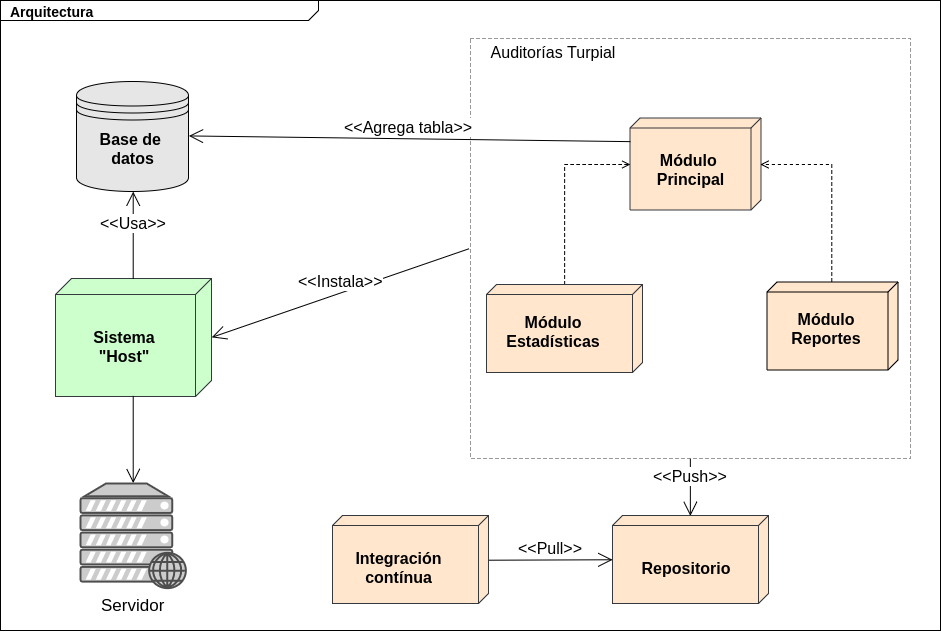
\includegraphics[width=\textwidth]{Diagrama_Arquitectura.png}
\caption{Arquitectura de la librería Auditorías Turpial}
\label{fig:figure6.1}
\end{figure}

Se decidió que el módulo Principal agregaría una nueva tabla en la base de datos ya existente del “Host” en la que mantendrá la información acerca de las auditorías y los otros módulos podrían leerla para procesarla y mostrarla como sea  pertinente.\\

No obstante, la arquitectura mostrada en la figura 6.1 sufrió modificaciones durante el desarrollo  el proyecto para simplificarla. En lugar de crear tres aplicaciones, una para cada módulo, se separó Auditorías Turpial en dos: \textit{backend} y \textit{frontend}. En la sección que explica la fase de construcción se ofrecerán mayores detalles de estos cambios y sus razones.

\begin{figure}
\centering
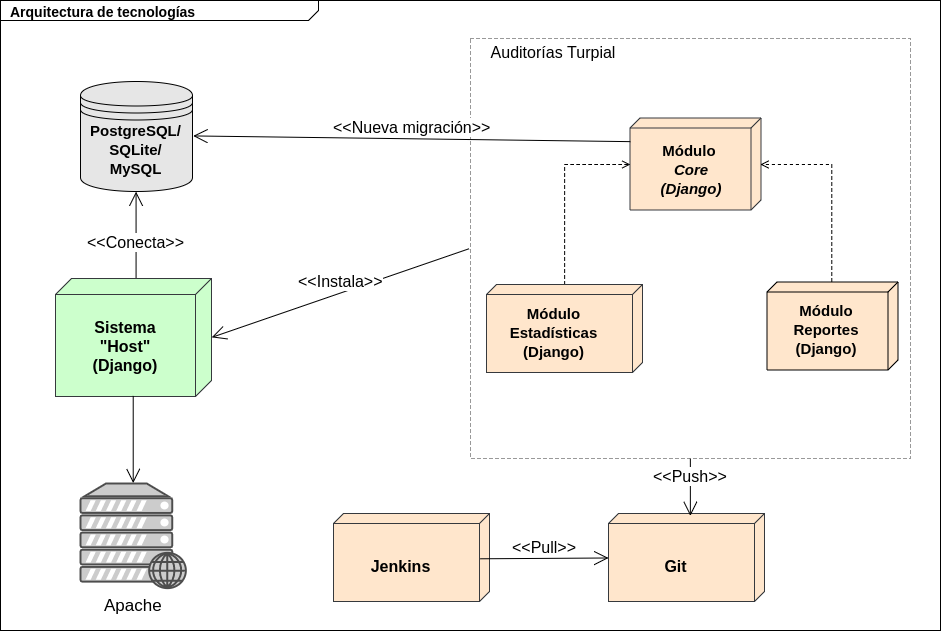
\includegraphics[width=\textwidth]{Diagrama_Tecnologias.png}
\caption{Arquitectura de tecnologías a utilizar}
\label{fig:figure6.2}
\end{figure}

En la figura 6.2 se muestran las tecnologías a utilizar en el proyecto. Como se mencionó anteriormente, se utilizará Django para el desarrollo. Como herramienta de control de versiones se utilizará Git y para automatizar la integración contínua se usará Jenkins. El sistema “Host” será un proyecto de la empresa que utilizará como servidor Web, Apache y una base de datos relacional.

\section{Diseño del módulo principal}

Uno de los problemas más significativos que la empresa encuentra en otras extensiones de Django disponibles, es el hecho de que el registro de auditoría se guarda a nivel de la vista y es responsabilidad del programador colocar el código para esta funcionalidad. Esto da cabida a que se olvide colocar en alguna de las vistas correspondientes a algún modelo, por lo que podría no guardarse todos los tipos de operaciones. \\

La librería Auditorías Turpial pretende evitar este problema guardando el registro de auditoría cada vez que ocurre alguna operación sobre el modelo a través del uso de las señales (\textit{signals}) que ofrece el \textit{framework} . Éstas señales, necesariamente deben distinguir entre un modelo auditable y uno que no lo es. Para esto, se contempló el uso de un \textit{mixin} que pueda ser heredado por cualquier modelo y así proveer todas las funcionalidades mencionadas. \\

Por otro lado, se desea incluir en las auditorías el usuario que realizó la acción. La solución mencionada anteriormente no es suficiente para lograr esto, puesto que a nivel de modelos no se posee información sobre el \textit{request} y no se puede saber qué usuario está en sesión. Por esta razón, se planteó agregar otro \textit{mixin} a nivel de vistas que completara la información antes de guardarla en la base de datos. Sería responsabilidad del programador heredarlo en todas las vistas cuyos modelos mantienen un historial de transacciones.
 \\

Django posee mecanismos para traducir los modelos a otro formato con una estructura bien definida, más conocidos como \textit{serializers} (serializadores), y viceversa. En particular, posee maneras de convertirlos a JSON, por lo que se decidió utilizar dicha funcionalidad para cumplir con el requisito de mostrar los cambios en los valores de los campos del modelo auditable en este formato.\\

En cuanto a los listados, se acordó utilizar Datatables para mostrarlos como una tabla que se pueda ordenar y filtrar fácilmente. Este \textit{plugin} puede manejar aproximadamente 10000 filas en sus tablas procesándolas del lado del cliente, sin embargo, las auditorías serán potencialmente millones de registros, es por esta razón se debe realizar el procesamiento del lado del servidor. \\

Para la autenticación se consideró utilizar un tabla de usuarios propia con su respectiva permisología, con la intención de que no interfiriera con la del sistema “Host”, sin embargo, esto no fue posible. Se ahondará en la explicación de esta decisión en la fase de desarrollo del presente capítulo.

\subsection{Diseño del módulo de estadísticas}

Uno de los requisitos mínimos con el que debe contar el módulo de Estadísticas es exponer un conjunto de gráficas que permitan visualizar e interpretar fácilmente los resultados de los cálculos de las auditorías. Para esto, se investigaron dos librerías de JavaScript: Amcharts y Charts.js. En la siguiente tabla se muestran las características principales:

%%%%% tabla%%%%

Como los desarrolladores de Turpial Development son los principales usuarios de este proyecto, el pasante investigó si existía alguna librería que utilicen usualmente. En la empresa han utilizado varias, incluyendo las dos presentadas anteriormente, por lo que no tienen una preferencia en este sentido. \\

Debido a que la cantidad de registros de auditorías pueden crecer rápidamente, es necesario escoger una librería de gráficos que maneje adecuadamente grandes volúmenes de datos, por lo que se decidió utilizar Amcharts. Otra característica que inclina la balanza a favor de esta solución, es el hecho de que posee un \textit{plugin} que permite exportar datos a un archivo CSV o PDF, una funcionalidad que se compenetra bien con el módulo de Reportes. \\

Aunque Charts.js posee una extensión de Django para facilitar la creación de los gráficos a través de las vistas, este proyecto requiere una lógica muy específica para entregar el conjunto de datos que se utilizará para renderizarlos. Por esta razón, es mejor tener total control sobre su implementación. \\

Los cálculos estadísticos serán entregados a la plantilla a través de una vista que incluirá el formulario de los filtros y la manipulación de los datos para crear los gráficos pertinentes y según los requiera la librería escogida.

\subsection{Propuesta para la integración continua}

Dado que en la empresa no existe precedente sobre el uso de una herramienta automatizada para integrar el código de manera continua, se le otorgó al pasante la libertad de escoger entre dos herramientas sugeridas por el líder del proyecto: Jenkins o Fabric. Para decidir cuál herramienta se adecuaba más al proyecto y a las necesidades de la empresa, fue indispensable que el pasante investigara las opciones en profundidad, sus fortalezas, limitaciones y recomendaciones de la comunidad. A continuación se muestra una comparación entre ellas:

%%% tabla%%%%

Considerando las características que posee cada herramienta, se decidió utilizar Jenkins puesto que se pueden ejecutar \textit{scripts} de manera programada, generar reportes, observar el estado del despliegue de varios proyectos e incluso integrarlo con Gitlab, un servicio Web de control de versiones y desarrollo de \textit{software} colaborativo basado en Git que es utilizado por la empresa. \\

Si bien Fabric es más simple, no es realmente un servidor para integración continua, se asemeja más a \textit{scripts} que permiten automatizar tareas y se requiere de una herramienta suficientemente general que pueda ser usado tanto en la pasantía como en otros proyectos de la empresa.

\subsection{Plan de pruebas}

Para verificar que cada funcionalidad posea el comportamiento esperado, se realizaron pruebas de manera automatizada utilizando Pytest. Más específicamente, se llevaron a cabo pruebas unitarias, de regresión y de integración.

Adicionalmente, se convino que uno de los criterios de aceptación de las HU era validar el producto con el cliente para asegurar el cumplimiento de las reglas de negocio y que el producto desarrollado cumple los estándares. A esto se le conoce como pruebas de aceptación y fueron realizadas en cada cierre de \textit{Sprint}.

Como el proyecto en cuestión es una librería, no puede funcionar por sí sola, sino que necesita instalarse en otro. Para esto, se creó una aplicación sencilla en Django y se instaló la librería en él. En cada \textit{Sprint}, se constató que el programador pueda usar cada funcionalidad desarrollada  sin ningún inconveniente. Este mismo proyecto, se utilizó para mostrar los avances al cliente.\\

En la fase de transición, se planificó que se realizaran pruebas en una aplicación desarrollada para uso interno de la empresa, llamado Turpial Team, cuyo propósito es gestionar empleados y permitir que conozcan a su equipo de trabajo. No obstante, debido a que aún se encuentra en desarrollo no está disponible actualmente. Se optó por utilizar otro proyecto de uso interno de Turpial Development, llamado Turpial Calendar. Esta aplicación sirve para planificar eventos de la empresa y enviar notificaciones. Esta decisión no afecta de ninguna manera la pasantía ya que la librería debe poder ser instalada en cualquier proyecto con las características mencionadas en la sección de requerimientos.

\subsection{Planificación del desarrollo del proyecto}

Luego de finalizar el proceso de investigación, aclarar los requerimientos y determinar las HU, se procedió a planificar la fase de construcción del proyecto. Para ello, se tomó en cuenta la prioridad, precedencia y puntaje de cada HU para determinar el orden. Se decidió iniciar con las HU relacionadas con el \textit{Core} y la instalación de la librería.\\

Se planificaron ocho \textit{Sprints} con una duración de dos semanas laborales (diez días) cada uno. Estos \textit{Sprints} abarcan la fase de construcción del módulo \textit{Core} y Estadísticas de Auditorías Turpial, así como la fase de transición.

\section{Fase de construcción}

Una vez culminada la fase de concepción, se procedió con la instalación del ambiente de desarrollo e implementación de los módulos que abarca la pasantía. También, se incluyen las pruebas pertinentes para cada funcionalidad desarrollada según indica el Plan de Pruebas.

\subsection{Módulo \textit{Core}}

En esta sección se describe el proceso para desarrollar cada HU relacionada con el módulo Core, los problemas encontrados y sus soluciones. También se explica el nuevo diseño de la arquitectura y las pruebas efectuadas.

\subsubsection{Estructura de la tabla de auditorías}

Antes de iniciar con la implementación de la librería, se instalaron y configuraron todas las herramientas necesarias para esto. En primer lugar, se instaló Python 2.7 y luego PIP. Se instaló el plugin de Python, Virtualenv, el cual permitió configurar el ambiente virtual. Este, se utilizó para instalar los requerimientos de la librería, en particular, Django y Pytest. Estos plugins se registraron en el archivo “requirements.txt” para facilitar futuras instalaciones y determinar las dependencias de la librería.\\

Luego, se procedió a crear la aplicación de Django y la estructura del módulo Core. Para ello, se utilizaron los comandos que posee el \textit{framework}, “startproject” y “startapp” respectivamente.

\section{Fase de construcción del módulo de estadísticas}
\section{Fase de transición}
  % Chapter 4: Title of the chapter
%----------------------------------------------------------------------------------------%

\addtocontents{toc}{\addvspace{.5cm}}
\addcontentsline{toc}{chapter}{\textbf{CONCLUSIONES}}
\chapter*{\textbf{CONCLUSIONES}}

\thispagestyle{empty}

\addcontentsline{toc}{section}{Conclusiones}
\section*{Conclusiones}

\addcontentsline{toc}{section}{Recomendaciones}
\section*{Recomendaciones}

%
%----------------------------Additional chapters may be added ---------------------------%
%                                                                                        %
%----------------------------------------------------------------------------------------%
% Bibliography on Chicago Thesis Style with modifications by Rand Alfaris.               %
% Don't make any changes on the following, except for the name of the bibliography file. %
% For example, we choose here a file named "bibli".                                      %
%----------------------------------------------------------------------------------------%
\addcontentsline{toc}{chapter}{\textbf{Referencias}}
% \pagestyle{fancy}
\begin{singlespace}
\bibliographystyle{apalike}
\bibliography{14_Referencias}
\end{singlespace}
%----------------------------------------------------------------------------------------%
\newpage
\addcontentsline{toc}{chapter}{\textbf{Apéndices}}
\appendix
% %  \refstepcounter{chapter}%
 \chapter*{APPENDIX \thechapter} \label{appendixA}
 \begin{center}
\textbf{ALGORITHMS}
\end{center}
% \refstepcounter{section}
\section*{\thesection \quad Simulated Annealing}

\begin{figure}[h!]
\begin{center}
\begin{footnotesize}
\begin{tabular}{|llll|}\hline%
    &     &     & \\%
\multicolumn{4}{|l|}{\textbf{Random decimal numbers} $g$ to $a$ and $T$ to $T_{0}$} \\%
\multicolumn{4}{|l|}{\textbf{Loop} - {\slshape Cooling}} \\%
    & \multicolumn{3}{l|}{\hspace{0.3cm} \textbf{Loop} - {\slshape Local Search}} \\%
    &     & \multicolumn{2}{l|}{\hspace{0.7cm} Derive a neighbour, $j$ of $i$} \\%
    &     & \multicolumn{2}{l|}{\hspace{0.7cm}$\triangle E:=E(j)-E(i)$ } \\%
    &     & \multicolumn{2}{l|}{\hspace{0.7cm} \textbf{If} $\triangle E < 0$} \\%
    &     & \multicolumn{2}{l|}{\hspace{0.7cm} \textbf{Then} $i:=j$} \\%
    &     & \multicolumn{2}{l|}{\hspace{0.7cm} \textbf{Else} derive random number $r \in [0,1]$} \\%
    &     &     &  \hspace{1.2cm} \textbf{If} $r < e^{ - \frac{{\Delta E}}{T}}$\\%
    &     &     &  \hspace{1.2cm} \textbf{Then} $i:=j$\\%
    &     &     &  \hspace{1.2cm} \textbf{End If} \\%
    &     & \multicolumn{2}{l|}{\hspace{0.7cm} \textbf{End If}} \\%
    & \multicolumn{3}{l|}{\hspace{0.3cm} \textbf{End Loop} -- {\slshape Local Search}} \\%
    & \multicolumn{3}{l|}{\hspace{0.3cm} \textbf{Exit} (when goal is satisf\mbox{}ied or the stopping criterion is reached)} \\%
    & \multicolumn{3}{l|}{\hspace{0.3cm} $T = C(T)$ } \\%
\multicolumn{4}{|l|}{\textbf{End Loop} -� {\slshape Cooling}} \\%
    &     &     & \\\hline%
\end{tabular}
\end{footnotesize}
{\bf{\caption{Algorithm of Simulated Annealing}}}\label{AlgSA}%
\end{center}
\addtocontents{lof}{\protect\addvspace{.5cm}}
\end{figure}

\newpage
\refstepcounter{section}
\section*{\thesection \quad Genetic Algorithm}

\begin{figure}[h!]
\begin{center}
\begin{small}
\begin{tabular}{|ll|}\hline%
\multicolumn{2}{|l|}{{\bf S1:}  \textbf{[Start]} Generate an initial population $P_{pop}$, of $n$ chromosomes.}\\%
\multicolumn{2}{|l|}{{\bf S2:}  \textbf{[Fitness]} Evaluate the f\mbox{}itness $g(x)$ of each chromosome $x$ in the population.}\\%
\multicolumn{2}{|l|}{{\bf S3:}  \textbf{[New Population]} Create a new population by repeating the following}\\%
           & \hspace{3.7cm} steps until the new population is complete.\\%
           & \hspace{0.3cm} i.   \textbf{[Selection]} Select 2 parent chromosomes from a population according\\%
           & \hspace{2.9cm}to their f\mbox{}itness (the f\mbox{}itter, the better chance of being selected).\\%
           & \hspace{0.3cm} ii.   \textbf{[Crossover]} With a crossover probability $p_{c}$, cross over the parents to\\%
           & \hspace{3.2cm}form 2 new of\mbox{}fspring (children). If no crossover was\\%
           & \hspace{3.2cm}performed, the of\mbox{}fspring is an exact copy of parents.\\%
           & \hspace{0.3cm} iii.  \textbf{[Mutation]} With a mutation probability $p_{m}$, mutate new of\mbox{}fspring at\\%
           & \hspace{3.2cm}each locus (position in chromosome).\\%
           & \hspace{0.3cm} iv.  \textbf{[Replace]} Place new of\mbox{}fspring in the new population.\\%
\multicolumn{2}{|l|}{{\bf S4:}  \textbf{[Fitness]} Evaluate the f\mbox{}itness $g(x')$ of each chromosome $x'$ in the new}\\%
           & \hspace{1.9cm} population.\\%
\multicolumn{2}{|l|}{{\bf S5:}  \textbf{[Test]} If the end condition is satisf\mbox{}ied, {\bf STOP}, and return the f\mbox{}ittest solution}\\%
           & \hspace{1.4cm} found; otherwise, go to {\bf S3}.\\\hline%
\end{tabular}
\end{small}
{\bf{\caption{Algorithm of a Genetic Algorithm}\label{AlgGA}}}%
\end{center}
\addtocontents{lof}{\protect\addvspace{.5cm}}
\end{figure}

\newpage
\refstepcounter{section}
\section*{\thesection \quad Tabu Search}

\begin{figure}[h!]
\begin{center}
\begin{scriptsize}
\begin{tabular}{|lllllll|}\hline%
   &    &    &    &    &    &\\%
\multicolumn{7}{|l|}{{\bf procedure} SEARCH$(t,k,diversify,z)$:} \\%
   & \multicolumn{6}{l|}{\hspace{0.3cm}$penalty^{*}:=+\infty$;} \\%
   & \multicolumn{6}{l|}{\hspace{0.3cm}{\bf for each} $j\in S_{t}$ {\bf do}} \\%
   &    & \multicolumn{5}{l|}{\hspace{0.6cm}{\bf for each} $k$-tuple $K$ of bins not including $t$ {\bf do}} \\%
   &    &    & \multicolumn{4}{l|}{\hspace{0.9cm}$S:=\{j\}\cup(\bigcup_{i\in K}S_{i})$;} \\%
   &    &    & \multicolumn{4}{l|}{\hspace{0.9cm}$penalty := +\infty$;} \\%
   &    &    & \multicolumn{4}{l|}{\hspace{0.9cm}{\bf case}} \\%
   &    &    &    & \multicolumn{3}{l|}{\hspace{1.2cm}$A(S) < k$:} \\%
   &    &    &    &    & \multicolumn{2}{l|}{\hspace{1.5cm}execute the move and update the solution value $z$;} \\%
   &    &    &    &    & \multicolumn{2}{l|}{\hspace{1.5cm}$k := \max\{1,k-1\}$;} \\%
   &    &    &    &    & \multicolumn{2}{l|}{\hspace{1.5cm}{\bf return;}} \\%
   &    &    &    & \multicolumn{3}{l|}{\hspace{1.2cm}$A(S) = k$:} \\%
   &    &    &    &    & \multicolumn{2}{l|}{\hspace{1.5cm}{\bf if} the move is not tabu {\bf or} $S_{t}\equiv\{j\}$ {\bf then}} \\%
   &    &    &    &    &    & \hspace{1.8cm}execute the move and update the solution value $z$; \\%
   &    &    &    &    &    & \hspace{1.8cm}{\bf if}  $S_{t}\equiv\{j\}$ {\bf then} $k:= \max\{1,k-1\}$; \\%
   &    &    &    &    &    & \hspace{1.8cm}{\bf return} \\%
   &    &    &    &    & \multicolumn{2}{l|}{\hspace{1.5cm}{\bf end if;}} \\%
   &    &    &    & \multicolumn{3}{l|}{\hspace{1.2cm}$A(S)=k+1$ {\bf and} $k>1$:} \\%
   &    &    &    &    & \multicolumn{2}{l|}{\hspace{1.5cm}let $I$ be the set of $k+1$ bins used by $A$;} \\%
   &    &    &    &    & \multicolumn{2}{l|}{\hspace{1.5cm}$\overline{t}:=\arg \min_{i\in I}\{\varphi(Si)\}$, $T:=(S_{t}\backslash\{j\})\cup S_{\overline{t}}$;} \\%
   &    &    &    &    & \multicolumn{2}{l|}{\hspace{1.5cm}{\bf if} $A(T)=1$ {\bf and} the move is not tabu {\bf then}} \\%
   &    &    &    &    &    & \hspace{1.8cm}$penalty:= \min\{\varphi(T),\min_{i\in I\backslash\{\overline{t}\}}\{\varphi(S_{i})\}\}$ \\%
   &    &    & \multicolumn{4}{l|}{\hspace{0.9cm}{\bf end case;}} \\%
   &    &    & \multicolumn{4}{l|}{\hspace{0.9cm}$penalty^{*} := \min\{penalty^{*},penalty\}$;} \\%
   &    & \multicolumn{5}{l|}{\hspace{0.6cm}{\bf end for;}} \\%
   & \multicolumn{6}{l|}{\hspace{0.3cm}{\bf end for;}} \\%
   & \multicolumn{6}{l|}{\hspace{0.3cm}{\bf if} $penalty^{*}\neq +\infty$ {\bf then} execute the move corresponding to $penalty^{*}$} \\%
   & \multicolumn{6}{l|}{\hspace{0.3cm}{\bf else if} $k=k_{\max}$ {\bf then} $diversify :=$ \texttt{true} {\bf else} $k := k+1$} \\%
\multicolumn{7}{|l|}{{\bf return.}} \\\hline%
\end{tabular}
\end{scriptsize}
{\bf{\caption{Unif\mbox{}ied Tabu Search: Procedure
SEARCH}}}\label{AlgUTS_search}
\addtocontents{lof}{\protect\addvspace{.5cm}}
\end{center}
\end{figure}
 % Appendix A: Title of the appendix
% \refstepcounter{chapter}%
 \chapter*{APPENDIX \thechapter} \label{appendixB}
 \begin{center}
\textbf{TABLES}
\end{center}
\refstepcounter{section}
\section*{\thesection \quad Complex Tables}

Example of complex table \ldots e.g. Table \ref{TypoMSP}

\begin{table}[h!]
\begin{center}
{\textbf{\caption {Typology of Machine Scheduling Problems}\label{TypoMSP}}}%
\addtocontents{lot}{\protect\addvspace{.5cm}}
\begin{footnotesize}
\vspace{0.5cm}
\begin{tabular}{|c@{}|l@{ }|l@{ }|}\hline%
\multicolumn{1}{|c|}{\bf Characteristic} & \multicolumn{1}{|c|}{\bf Symbol} & \multicolumn{1}{|c|}{\bf Description}\\ \hline%
                 & $\alpha_{1}=\circ$      & a single machine \\%
                 & $\alpha_{1}=P$          & identical parallel machines \\%
                 & $\alpha_{1}=Q$          & uniform parallel machines \\%
         Machine & $\alpha_{1}=R$          & unrelated parallel machines \\%
     Environment & $\alpha_{1}=F$          & a f\mbox{}low shop \\%
        $\alpha$ & $\alpha_{1}=O$          & an open shop \\%
                 & $\alpha_{1}=J$          & a job shop \\\cline{2-3}%
                 & $\alpha_{2}=\circ$      & the number of machines is arbitrary \\%
                 & $\alpha_{2}=m$          & there are a f\mbox{}ixed number of machines $m$ \\\hline%
                 & $\beta_{1}=\circ$       & no release dates are specif\mbox{}ied \\%
                 & $\beta_{1}=r_{j}$       & jobs have release dates \\\cline{2-3}%
                 & $\beta_{2}=\circ$       & no deadlines are specif\mbox{}ied \\%
                 & $\beta_{2}=\bar{d}_{j}$ & jobs have deadlines \\\cline{2-3}%
             Job & $\beta_{3}=\circ$       & there are no setup times \\%
 Characteristics & $\beta_{3}=s_{ifg}$     & there are general family setup times \\%
         $\beta$ & $\beta_{3}=s_{fg}$      & there are machine independent family setup times \\%
                 & $\beta_{3}=s_{if}$      & there are sequence independent family setup times \\%
                 & $\beta_{3}=s_{f}$       & there are machine and sequence independent family setup times \\\cline{2-3}%
                 & $\beta_{4}=\circ$       & no precedence constraints are specif\mbox{}ied \\%
                 & $\beta_{4}=prec$        & jobs have precedence constraints \\%
                 & $\beta_{4}=pmtn$        & preemption of jobs is allowed\\\hline%
      Optimality & $C_{\max}$              & maximum completion time \\%
       Criterion & $L_{\max}$              & maximum lateness \\%
        $\gamma$ & $\mathop{\sum}\limits_j (w_{j})C_{j}$     & total (weighted) completion time \\%
                 & $\mathop{\sum}\limits_j (w_{j})T_{j}$     & total (weighted) tardiness \\%
   (involves the & $\mathop{\sum}\limits_j (w_{j})U_{j}$     & total (weighted) number of late jobs \\%
minimisation of) & $\mathop{\sum}\limits_j (w_{j})E_{j}$     & total (weighted) earliness \\ \hline%
\end{tabular}
\end{footnotesize}
\end{center}
\end{table}

Example of landscape (or sideway) table \ldots e.g. Table
\ref{Lmax_Bin}
\begin{sidewaystable}[h!]
\begin{center}
{\textbf{\caption{A Comparison of Dif\mbox{}ferent Local Search
Algorithms}\label{Lmax_Bin}}}
\addtocontents{lot}{\protect\addvspace{.5cm}}
\begin{scriptsize}
\vspace{0.5cm}
\begin{tabular}{|c|c|c|c|r|c|c|r|c|c|r|c|c|r|}\hline%
Due Date   &  Data & \multicolumn{3}{|c|}{\textbf{SGA}} & \multicolumn{3}{|c|}{\textbf{$\textrm{MXGA}_{F}$}} &%
                    \multicolumn{3}{|c|}{\textbf{$\textrm{UTS}_{LGF}$}} & \multicolumn{3}{|c|}{\textbf{RDM}} \\\cline{3-14}%
     Class & Class & Ratio &   OBU & \multicolumn{1}{|c|}{ARD} & Ratio &   OBU & \multicolumn{1}{|c|}{ARD} &
                     Ratio &   OBU & \multicolumn{1}{|c|}{ARD} & Ratio &   OBU & \multicolumn{1}{|c|}{ARD} \\\hline%
           &     I & 1.056 & 83.10 &   16.58 & 1.042 & 85.26 &   12.37 & 1.053 & 83.42 &   16.02 & 1.088 & 78.73 &   22.27 \\%
           &    II & 1.033 & 63.69 &   17.38 & 1.020 & 66.19 &   11.15 & 1.025 & 64.92 &   13.17 & 1.025 & 65.36 &   12.00 \\%
           &   III & 1.109 & 71.36 &   30.86 & 1.078 & 75.40 &   22.00 & 1.084 & 74.51 &   27.90 & 1.092 & 73.23 &   26.59 \\%
           &    IV & 1.047 & 60.68 &   21.74 & 1.047 & 61.65 &   17.29 & 1.033 & 62.25 &   19.09 & 1.040 & 61.77 &   18.95 \\%
\textbf{A} &     V & 1.087 & 72.45 &   24.24 & 1.070 & 74.46 &   18.00 & 1.077 & 73.61 &   21.97 & 1.076 & 73.53 &   21.73 \\%
           &    VI & 1.110 & 54.51 &   23.23 & 1.093 & 56.01 &   16.66 & 1.110 & 54.41 &   21.49 & 1.103 & 55.34 &   19.34 \\%
           &   VII & 1.120 & 74.45 &   33.48 & 1.090 & 78.54 &   23.52 & 1.107 & 76.70 &   29.67 & 1.099 & 77.10 &   29.46 \\%
           &  VIII & 1.125 & 74.14 &   33.96 & 1.089 & 78.79 &   23.31 & 1.102 & 77.26 &   29.99 & 1.103 & 76.41 &   29.03 \\%
           &    IX & 1.007 & 44.07 &    1.68 & 1.007 & 44.10 &    1.68 & 1.007 & 42.92 &    1.74 & 1.007 & 43.17 &    2.12 \\%
           &     X & 1.099 & 74.96 &   27.90 & 1.080 & 77.27 &   23.89 & 1.089 & 76.59 &   32.05 & 1.093 & 74.93 &   27.54 \\\hline%
\multicolumn{2}{|c|}{\textbf{Average}} & 1.079 & 67.34 & 23.10 & \textbf{1.062} & \textbf{69.77} & \textbf{16.99}%
                                       & 1.069 & 68.66 & 21.31 & 1.073 & 67.96 & 20.90 \\\hline\hline%
           &     I & 1.065 & 81.82 &   34.93 & 1.046 & 84.73 &   24.17 & 1.069 & 81.58 &   31.78 & 1.088 & 78.46 &   38.27 \\%
           &    II & 1.033 & 63.61 &   47.72 & 1.027 & 65.52 &   33.98 & 1.038 & 64.05 &   39.68 & 1.032 & 63.68 &   33.46 \\%
           &   III & 1.132 & 68.91 &   66.78 & 1.088 & 73.90 &   46.21 & 1.128 & 69.99 &   64.99 & 1.107 & 71.50 &   56.46 \\%
           &    IV & 1.060 & 59.27 &   53.45 & 1.047 & 61.70 &   35.98 & 1.063 & 59.58 &   49.09 & 1.060 & 59.22 &   45.72 \\%
\textbf{B} &     V & 1.113 & 69.66 &   48.58 & 1.080 & 73.43 &   35.51 & 1.104 & 70.91 &   48.33 & 1.094 & 71.59 &   40.41 \\%
           &    VI & 1.110 & 54.34 &   48.85 & 1.110 & 54.93 &   37.73 & 1.090 & 55.34 &   46.41 & 1.097 & 55.00 &   42.01 \\%
           &   VII & 1.133 & 72.88 &   71.94 & 1.102 & 76.80 &   52.17 & 1.135 & 73.47 &   65.82 & 1.122 & 74.28 &   58.16 \\%
           &  VIII & 1.143 & 72.19 &   72.72 & 1.099 & 77.38 &   49.41 & 1.122 & 75.08 &   67.28 & 1.118 & 74.27 &   60.49 \\%
           &    IX & 1.007 & 43.84 &    2.42 & 1.007 & 43.97 &    2.42 & 1.007 & 43.09 &    2.53 & 1.007 & 43.30 &    3.79 \\%
           &     X & 1.113 & 73.38 &   67.45 & 1.087 & 76.31 &   53.48 & 1.125 & 72.90 &   81.02 & 1.110 & 73.23 &   64.39 \\\hline%
\multicolumn{2}{|c|}{\textbf{Average}} & 1.091 & 65.99 & 51.48 & \textbf{1.069} & \textbf{68.87} & \textbf{37.11}%
                                       & 1.088 & 66.60 & 49.69 & 1.084 & 66.45 & 44.32 \\\hline\hline%
           &     I & 1.085 & 79.30 &  136.69 & 1.054 & 83.50 &   92.98 & 1.083 & 79.76 &  115.41 & 1.104 & 76.50 &  128.02 \\%
           &    II & 1.050 & 61.80 &  232.20 & 1.040 & 64.02 &  149.48 & 1.048 & 62.60 &  165.41 & 1.040 & 62.44 &  179.75 \\%
           &   III & 1.164 & 65.80 &  180.45 & 1.093 & 73.28 &  124.96 & 1.148 & 68.01 &  173.81 & 1.127 & 69.10 &  148.03 \\%
           &    IV & 1.070 & 58.68 &  223.21 & 1.053 & 60.59 &  153.24 & 1.063 & 60.12 &  210.69 & 1.063 & 59.19 &  183.06 \\%
\textbf{C} &     V & 1.134 & 67.32 &  149.25 & 1.088 & 72.38 &  105.04 & 1.134 & 68.20 &  142.07 & 1.106 & 69.88 &  121.12 \\%
           &    VI & 1.110 & 54.34 &  274.92 & 1.110 & 54.43 &  241.31 & 1.110 & 54.42 &  264.36 & 1.117 & 53.73 &  251.38 \\%
           &   VII & 1.161 & 70.18 &  296.58 & 1.106 & 76.20 &  209.59 & 1.164 & 70.42 &  261.95 & 1.134 & 71.77 &  227.27 \\%
           &  VIII & 1.153 & 70.86 &  421.53 & 1.101 & 76.79 &  273.28 & 1.172 & 69.72 &  387.14 & 1.135 & 72.15 &  320.40 \\%
           &    IX & 1.007 & 43.71 &    9.93 & 1.007 & 43.81 &    9.93 & 1.008 & 43.14 &   15.13 & 1.008 & 43.29 &   18.72 \\%
           &     X & 1.131 & 71.33 &  396.65 & 1.100 & 75.24 &  318.50 & 1.148 & 70.83 &  412.62 & 1.134 & 70.87 &  345.31 \\\hline%
\multicolumn{2}{|c|}{\textbf{Average}} & 1.107 & 64.33 & 232.14 & \textbf{1.075} & \textbf{68.02} & \textbf{167.83}%
                                       & 1.108 & 64.72 & 214.86 & 1.097 & 64.89 & 192.31 \\\hline%
\end{tabular}
\end{scriptsize}
\end{center}
\end{sidewaystable}
 % Appendix A: Title of the appendix           
%
%---------------------------Additional Appendices may be added---------------------------%
%                                                                                        %
%----------------------------------------------------------------------------------------%

% \addcontentsline{toc}{chapter}{\textbf{BIODATA OF STUDENT}}
% \include{biodata}   % Biodata of student                                                 %
% \addcontentsline{toc}{chapter}{\textbf{LIST OF PUBLICATIONS}}
% \include{listofpublications} % List of publications                                      %
\end{document}
%----------------------------------------------------------------------------------------%
